\documentclass[12pt, a4paper, oneside]{report}
\usepackage[lmargin=0.75in, rmargin=0.75in, tmargin=0.5in, bmargin=0.5in]{geometry}


\usepackage[english]{babel}
\usepackage[utf8]{inputenc}


\usepackage{graphicx}
\usepackage{subfig}
% \usepackage{cleveref}

\usepackage{caption}


\usepackage{lipsum}
\usepackage{titlesec}

\titleformat{\chapter}[display]
  {\normalfont\bfseries}{}{0pt}{\Huge}
  
\usepackage{enumitem}

\usepackage{url} 

\usepackage{amsmath}    

\usepackage{float}
\usepackage{multirow}
\usepackage{siunitx}


\usepackage{color}   %May be necessary if you want to color links
\usepackage{hyperref}
\hypersetup{
    colorlinks=true, %set true if you want colored links
    linktoc=all,     %set to all if you want both sections and subsections linked
    linkcolor=blue,  %choose some color if you want links to stand out
}

\usepackage[toc,page]{appendix}
% Your document starts here!
\begin{document}



\begin{titlepage}

\newcommand{\HRule}{\rule{\linewidth}{0.5mm}} % Defines a new command for the horizontal lines, change thickness here

\center % Center everything on the page
 
%----------------------------------------------------------------------------------------
%	HEADING SECTIONS
%----------------------------------------------------------------------------------------


\textsc{\large Indian Institute of Technology Madras}\\[0.5cm]

\HRule \\[0.8cm]
{ \large \bfseries Project 3}\\[0.4cm]
% Title of your document
{ \large \bfseries Suspension Control}\\[0.2cm]
\HRule \\[1.5cm]
 
%----------------------------------------------------------------------------------------
%	AUTHOR SECTION
%----------------------------------------------------------------------------------------

\begin{minipage}{0.8\textwidth}
\begin{center} \large
{ED5330}\\
\emph{Course Instructor: Prof Srikanthan }\\


\end{center}



\end{minipage}

\bigskip
\bigskip

\emph{Members: }\\
\begin{center} \large
    Adil Mohammed K ED19B041\\
    Benny SL ME19B087 \\
    
   
    
    
\end{center}

\begin{figure}[h]
\centerline{
\includegraphics[scale=0.6]{logo_iitm.png}}

\label{logo}
\end{figure}

\begin{center}\large
    {Odd Semester July - November 2022}
\end{center}


\end{titlepage}



\newpage

\tableofcontents


\chapter{Introduction}

Suspension systems are a integral part in ride comfort and handling of a vehicle.
Using this paper, we will try to answer the following questions:
\begin{itemize}
    \item System modelling
    \begin{itemize}
        \item Derive the equations of motion of this System
        \item Calculate the natural frequencies of the system
        \item State-Space representation of the system
    \end{itemize}
    \item Open-loop Suspension Performance Analysis
    \begin{itemize}
        \item Derive three transfer function
        \item Bode plot of the transfer functions for multiple parameters
    \end{itemize}
    \item Closed-loop Suspension Performance Analysis
    \begin{itemize}
        \item Develop a Linear Quadratic Regulator (LQR)
        \item Calculate the optimal regulator gain
        \item plot the Bode diagram of each of the three transfer functions, with and without control.
    \end{itemize}
\end{itemize}

\chapter{Quarter Car Modelling}
\section{Governing Equations}

\begin{figure}[h]
        \centering
        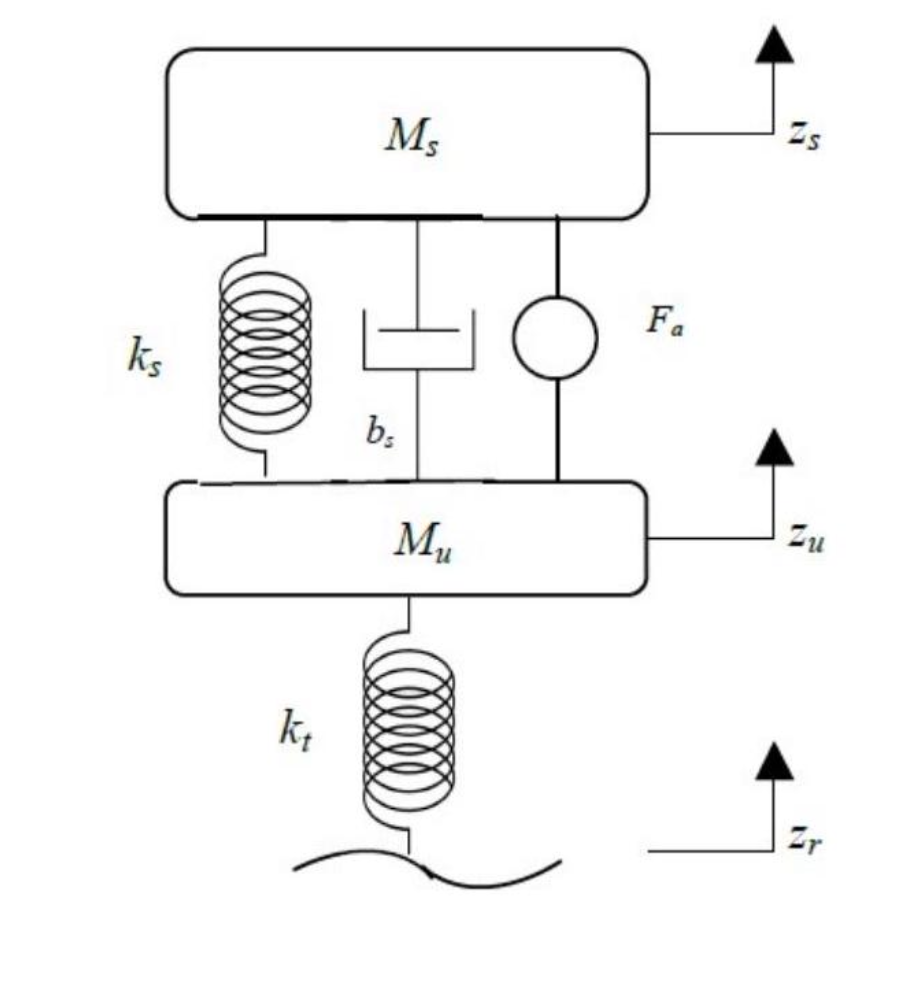
\includegraphics[width=0.5\textwidth]{images/quarter_model.png}
        \caption{Quarter Model}
    \end{figure}

Let the parameters be:
\begin{itemize}
    \item  $M_s$: Sprung Mass
    \item $M_u$: Unsprung mass
    \item $k_s$: Suspension stiffness
    \item $k_t$: Tyre stiffness
    \item $b_s$: Suspension damping 
\end{itemize}

\subsection{Equations of Motion}
Considering the sprung mass, applying force balance

\begin{equation}
    \begin{aligned}
        m_s \ddot{z_s} = -k_s (z_s - z_u) - b_s (\dot{z_s} - \dot{z_u}) + F_a \\
        m_s \ddot{z_s} + b_s (\dot{z_s} + k_s z_s = F_a + b_s \dot{z_u} + k_s z_u
    \end{aligned}
\end{equation}

Considering the unsprung mass, applying force balance

\begin{equation}
    \begin{aligned}
        m_u \ddot{z_u} = k_s (z_s - z_u) + b_s (\dot{z_s} - \dot{z_u}) - F_a - k_t (z_u - z_r) \\
        m_s \ddot{z_u} + b_s (\dot{z_u} + (k_s + k_t) z_u + F_a = b_s \dot{z_s} + k_s z_s + k_t z_r
    \end{aligned}
\end{equation}

The above equations can be written as:

\begin{equation}
    \begin{aligned}
        \begin{bmatrix}
            m_s & 0 \\
            0 & m_u
        \end{bmatrix}
        \begin{bmatrix}
            \ddot{z_s} \\
            \ddot{z_u}
        \end{bmatrix}
        +
        \begin{bmatrix}
            b_s & -b_s \\
            -b_s & -b_s
        \end{bmatrix}
        \begin{bmatrix}
            \dot{z_s} \\
            \dot{z_u}
        \end{bmatrix}
        +
        \begin{bmatrix}
            k_s & -k_s \\
            -k_s & k_s + k_t
        \end{bmatrix}
        \begin{bmatrix}
            z_s \\
            z_u
        \end{bmatrix}
        =
        \begin{bmatrix}
            0 \\
            k_t
        \end{bmatrix} z_r
        +
        \begin{bmatrix}
            1 \\
            -1
        \end{bmatrix} F_a
    \end{aligned}
\end{equation}

\begin{equation}
    M \ddot{z} + C \dot{z} + K z = B_1 z_r + B_1 F_a
\end{equation}

\subsection{Natural Frequencies}

\paragraph[]{Natural Frequencies of the system} can be calculated using the following formula:


\begin{align}
        \left\lvert -\omega_n^2 M + K  \right\rvert = 0 \\
        \begin{vmatrix}
            -\omega_n^2 m_s + k_s & -k_s \\
            -k_s & -\omega_n^2 m_u + k_s + k_t
        \end{vmatrix} \nonumber
        = 0 \\
\end{align}


\begin{equation}
    m_s m_u \omega_n^4 -( m_s(k_s + k_t) + m_u k_s) \omega_n^2 + k_s k_t = 0 
\end{equation}

On solving for $\omega_n^2$, we get:
\begin{equation}
    \omega_n^2 = \frac{k_s +k_t}{2m_u} + \frac{k_s}{2 m_s} \pm \left( \frac{\sqrt{(k_s +k_t)^2 m_s^2 + k_s^2 m_u^2 - 2( k_t - k_s)}m_s}{2 m_s m_u} \right)
\end{equation}

Substituting the values, we get 
\begin{equation}
    M = \begin{bmatrix}
        300 & 0 \\
        0 & 40
        \end{bmatrix} \text{and } K = \begin{bmatrix}
        15000 & -15000 \\
        -15000 & 165000
        \end{bmatrix}
        \nonumber
\end{equation}


We get $ \omega_n = 7.67 , 77.07$ rad/s.

\subsection{State-Space Representation of the system}

Let the state vector be $X = \begin{bmatrix}
    z_s -z_u \\
    \dot z_s \\
    z_u - z_r \\
    \dot z_u
    \end{bmatrix}$


\begin{align}
        \ddot{z_s} & = \frac{F_a}{m_s} - \frac{b_s}{m_s} \dot{z_s} + \frac{b_s}{m_s} \dot{z_u}- \frac{k_s}{m_s} (z_s - z_u) \\
        \ddot{z_u} & = -\frac{F_a}{m_u} - \frac{b_s}{m_u} \dot{z_u} + \frac{b_s}{m_u} \dot{z_s} + \frac{k_s}{m_u} (z_s - z_u) - \frac{k_t}{m_u} (z_u - z_r) 
\end{align}


Hence, the state-space representation of the system is:
\begin{equation}
    \dot X = \begin{bmatrix}
        0 & 1 & 0 & -1 \\
        -\frac{k_s}{m_s} & -\frac{b_s}{m_s} & 0 & -\frac{b_s}{m_s} \\
        0 & 0 & 0 & 1 \\
        \frac{k_s}{m_u} & \frac{b_s}{m_u} & -\frac{k_t}{m_u} & -\frac{b_s}{m_u} 
    \end{bmatrix}
    X + \begin{bmatrix}
        0 \\
        \frac{1}{m_s} \\
        0 \\
        -\frac{1}{m_u}
    \end{bmatrix} F
    + \begin{bmatrix}
        0 \\
        0 \\
        -1 \\
        0
    \end{bmatrix} \dot Z_r \\
\end{equation}
\begin{equation}
    \dot X = AX + bF + I \dot{z_r}
\end{equation}

\section{Open Loop Suspension Analysis}

\subsection{Open Loop Equations}


\subsubsection{Acceleration Transfer Function}
    \begin{equation}
        T_a(s) = \frac{L(\ddot{z_s(t)})}{L(\dot{z_r(t)})}
    \end{equation}
    Since we are considering passive suspension, $F_a = 0$.
    \begin{equation}
        \dot X = \begin{bmatrix}
            0 & 1 & 0 & -1 \\
            -\frac{k_s}{m_s} & -\frac{b_s}{m_s} & 0 & -\frac{b_s}{m_s} \\
            0 & 0 & 0 & 1 \\
            \frac{k_s}{m_u} & \frac{b_s}{m_u} & -\frac{k_t}{m_u} & -\frac{b_s}{m_u} 
        \end{bmatrix}
        X + \begin{bmatrix}
            0 \\
            0 \\
            -1 \\
            0
        \end{bmatrix} \dot Z_r \\
    \end{equation}
    \begin{equation}
        \ddot{z_r} = Y = \begin{bmatrix}
            -k_s/m_s & -b_s/m_s & 0 & b_s/m_s \\
        \end{bmatrix} X
    \end{equation}
    % \linebreak
    Where we have $u = \dot z_r(t)$ and 
    \begin{equation}
            A = \begin{bmatrix}
                0 & 1 & 0 & -1 \\
                -\frac{k_s}{m_s} & -\frac{b_s}{m_s} & 0 & -\frac{b_s}{m_s} \\
                0 & 0 & 0 & 1 \\
                \frac{k_s}{m_u} & \frac{b_s}{m_u} & -\frac{k_t}{m_u} & -\frac{b_s}{m_u}
            \end{bmatrix} \text{and } B = \begin{bmatrix}
                0 \\
                0 \\
                -1 \\
                0
            \end{bmatrix} 
            ,C = \begin{bmatrix}
                -k_s/m_s & -b_s/m_s & 0 & b_s/m_s \\
            \end{bmatrix}
            ,D = 0
            \nonumber
    \end{equation}

    Using MATLAB scripts, we get the following output.
\begin{figure}[h]
    \centering
    
    \subfloat[MATLAB Parameters]{\label{fig:open_loop1_Matlab}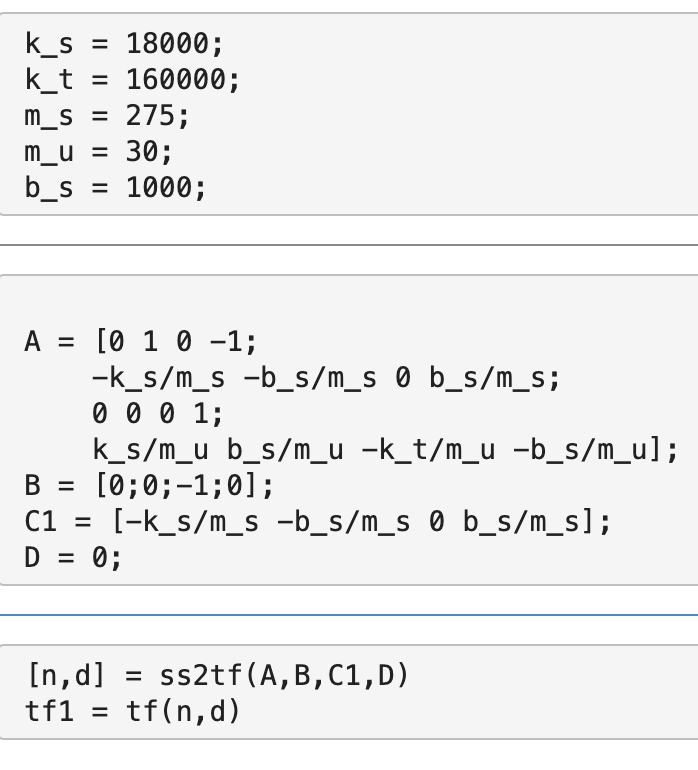
\includegraphics[width=.3\linewidth]{images/Q21_matlab.png}}\hfill
    \subfloat[Acceleration Transfer Function]{\label{fig:open_loop1_Matlab_eqn}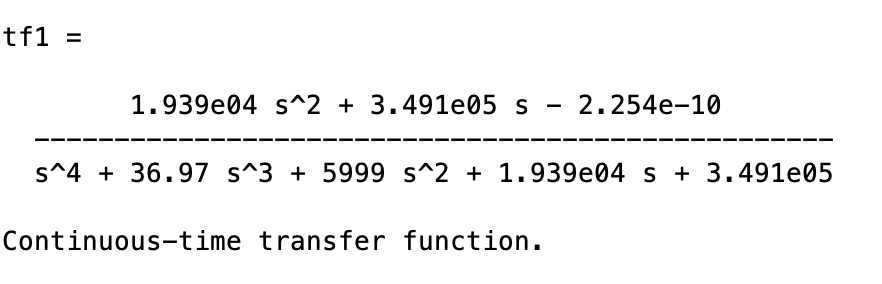
\includegraphics[width=.6\linewidth]{images/Q21_matlab_treqn.png}}\par 
    \caption{Acceleration Transfer Function calculation}
    \label{fig: open_loop1}
\end{figure}

\begin{equation}
    \label{eq:open_loop1}
    T_a(s) = \frac{ 19390 s^2 + 349100 s - 2.254 *10^{-10}}{s^4 + 36.97 s^3 + 5999 s^2 + 19390 s + 349100}
\end{equation}

\subsubsection{Rattle Transfer Function:}
    \begin{equation}
        T_r(s) = \frac{L(z_s(t) - z_u(t))}{L(\dot{z_r(t)})}
    \end{equation}

    \begin{equation}
        A = \begin{bmatrix}
            0 & 1 & 0 & -1 \\
            -\frac{k_s}{m_s} & -\frac{b_s}{m_s} & 0 & -\frac{b_s}{m_s} \\
            0 & 0 & 0 & 1 \\
            \frac{k_s}{m_u} & \frac{b_s}{m_u} & -\frac{k_t}{m_u} & -\frac{b_s}{m_u}
        \end{bmatrix} \text{and } B = \begin{bmatrix}
            0 \\
            0 \\
            -1 \\
            0
        \end{bmatrix} 
        ,C = \begin{bmatrix}
            1 & 0 & 0 & 0 \\
        \end{bmatrix}
        ,D = 0
        \nonumber
\end{equation}
\\
    Using MATLAB scripts, we get the following output.

\begin{figure}[H]
    \centering
    
    \subfloat[MATLAB Parameters]{\label{fig:open_loop2_Matlab}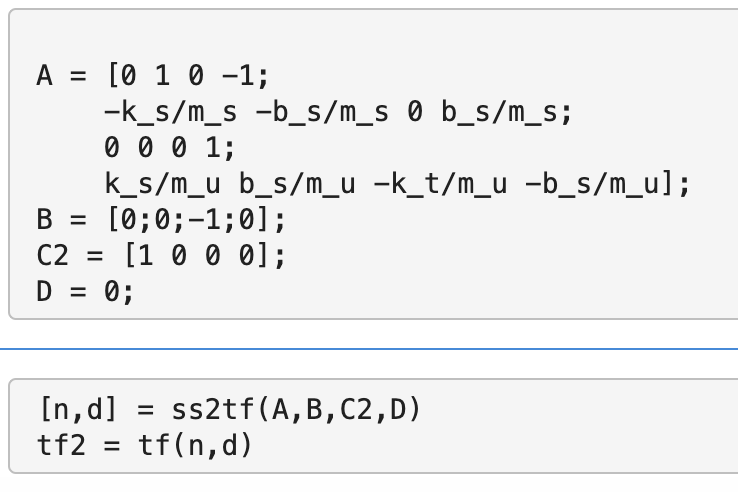
\includegraphics[width=.3\linewidth]{images/Q22_matlab.png}}\hfill
    \subfloat[Rattle Transfer Function]{\label{fig:open_loop2_Matlab_eqn}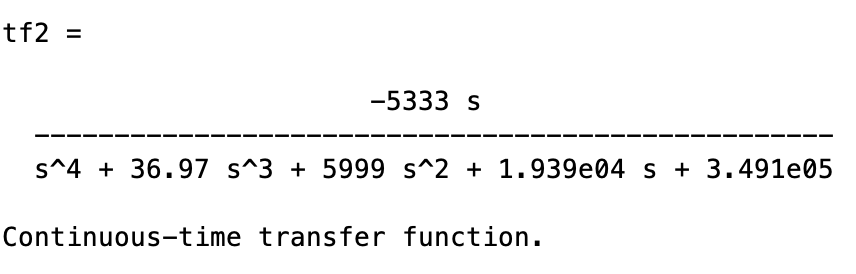
\includegraphics[width=.6\linewidth]{images/Q22_matlab_treqn.png}}\par 
    \caption{Rattle Transfer Function calculation}
    \label{fig: open_loop2}
\end{figure}

\begin{equation}
    \label{eq:open_loop2}
    T_r(s) = \frac{ -5333 s}{s^4 + 36.97 s^3 + 5999 s^2 + 19390 s + 349100}
\end{equation}

\subsubsection{Tyre Deflection Transfer Function}

\begin{equation}
    T_t(s) = \frac{L(z_u(t) - z_r(t))}{L(\dot{z_r(t)})}
\end{equation}

\begin{equation}
    A = \begin{bmatrix}
        0 & 1 & 0 & -1 \\
        -\frac{k_s}{m_s} & -\frac{b_s}{m_s} & 0 & -\frac{b_s}{m_s} \\
        0 & 0 & 0 & 1 \\
        \frac{k_s}{m_u} & \frac{b_s}{m_u} & -\frac{k_t}{m_u} & -\frac{b_s}{m_u}
    \end{bmatrix} \text{and } B = \begin{bmatrix}
        0 \\
        0 \\
        -1 \\
        0
    \end{bmatrix} 
    ,C = \begin{bmatrix}
        0 & 0 & 1 & 0 \\
    \end{bmatrix}
    ,D = 0
    \nonumber
\end{equation}
\\
Using MATLAB scripts, we get the following output.

\begin{figure}[H]
\centering

\subfloat[MATLAB Parameters]{\label{fig:open_loop3_Matlab}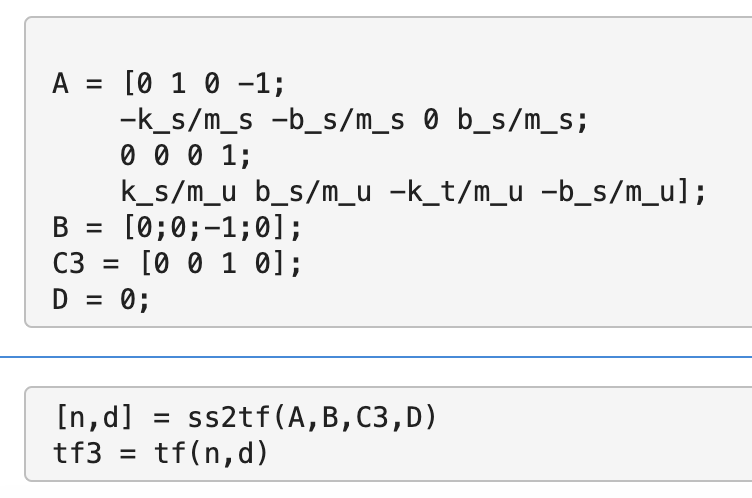
\includegraphics[width=.3\linewidth]{images/Q23_matlab.png}}\hfill
\subfloat[Tyre Deflection Transfer Function]{\label{fig:open_loop3_Matlab_eqn}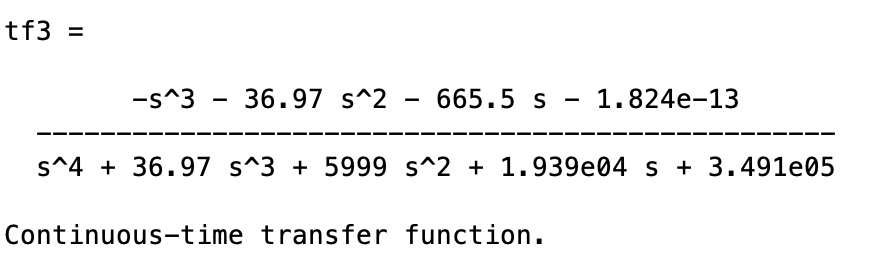
\includegraphics[width=.6\linewidth]{images/Q23_matlab_treqn.png}}\par 
\caption{Tyre Transfer Function calculation}
\label{fig: open_loop3}
\end{figure}

\begin{equation}
\label{eq:open_loop3}
T_t(s) = \frac{ -s^3 - 36.97 s^2 - 665.5 s - 1.824*10^{-13}}{s^4 + 36.97 s^3 + 5999 s^2 + 19390 s + 349100}
\end{equation}

\subsection{Bode Plots}

\begin{figure}[H]
\centering
\subfloat[][Acceleration Transfer Function Bode]{\label{fig:open_loop1_bode}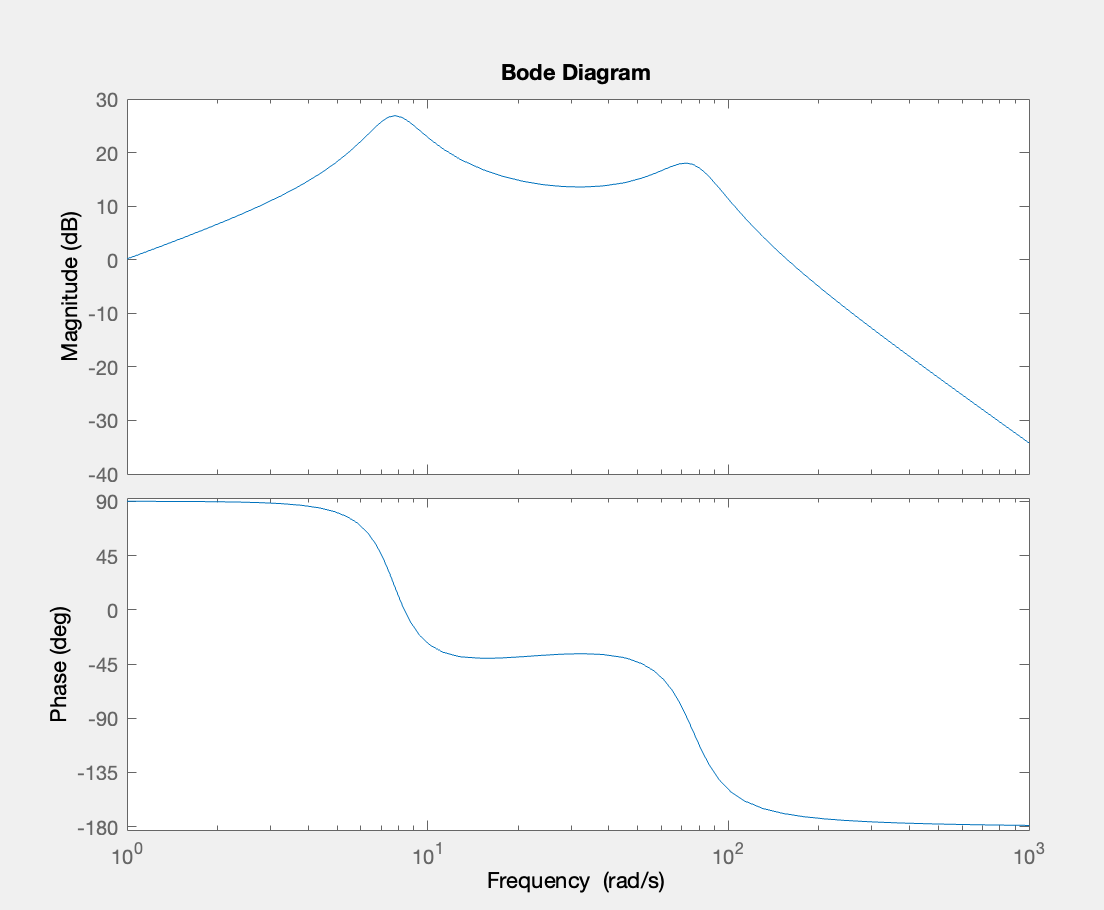
\includegraphics[width=.5\linewidth]{images/Q21_bode.png}}\hfill
\subfloat[][Rattle Transfer Function Bode]{\label{fig:open_loop2_bode}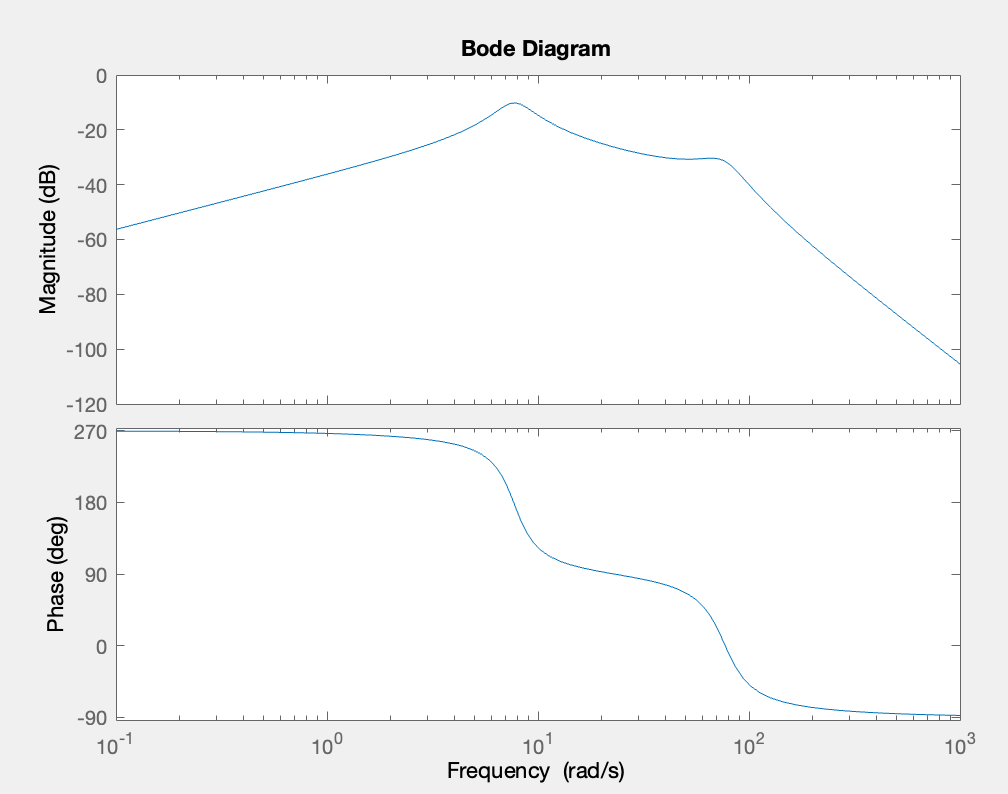
\includegraphics[width=.5\linewidth]{images/Q22_bode.png}}\hfill
\subfloat[][Tyre Transfer Function]{\label{fig:open_loop3_bode}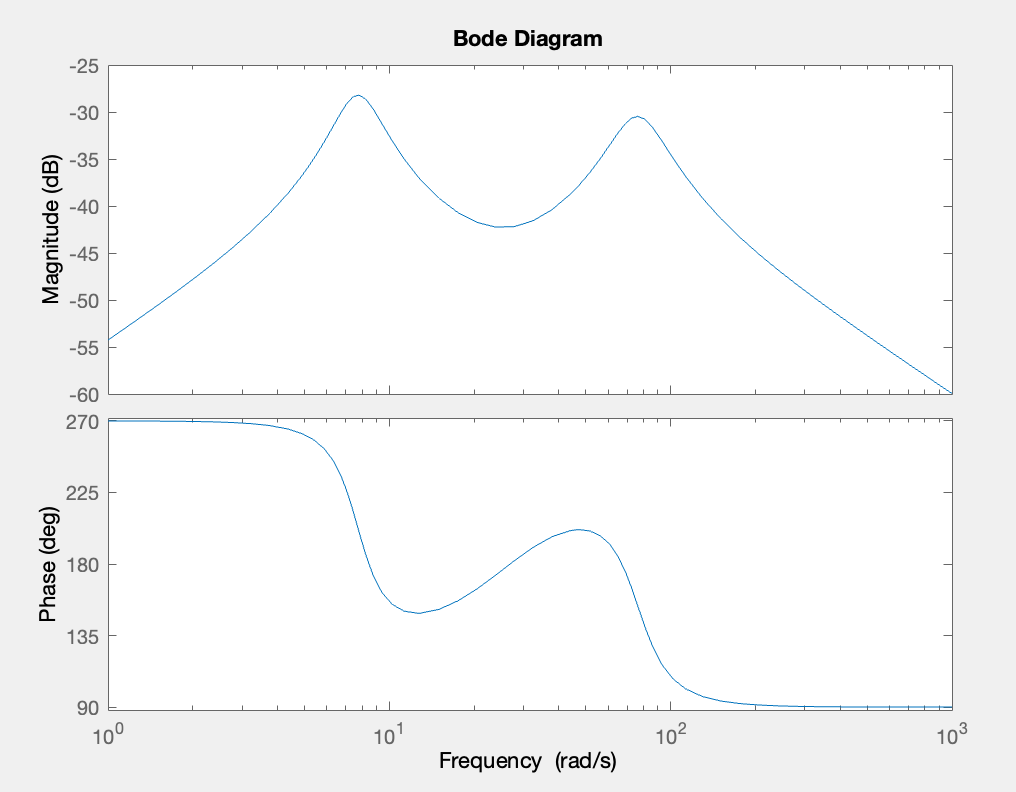
\includegraphics[width=.5\linewidth]{images/Q23_bode.png}}\par
\caption{Bode Plots}
\label{fig: open_loop_bode}
\end{figure}

\textbf{Observations:}
\begin{itemize}
    \item All the three transfer functions have the same natural frequencies, which can be confirmed by observing the maxima of three plots. All maxima occur at the same
    frequencies.
    \item The first peak of the plot corresponds to the resonance of the input with the spring
    damper system of the suspension of the vehicle and the second peak corresponds to that of the tyre's effective spring.
\end{itemize}

\subsection{Effect of Suspension Stiffness}


    For $k_s = 12000 N/m$ 

    $A = \begin{bmatrix}
        0 & 1 & 0 & -1 \\
        -43.6 & -3.6 & 0 & 3.6 \\
        0 & 0 & 0 & 1 \\
        400 & 33.3 & -5333.3 & -33.3
    \end{bmatrix}$\hfill \break

    For $k_s = 18000 N/m$ 

    $A = \begin{bmatrix}
        0 & 1 & 0 & -1 \\
        -43.6 & -3.6 & 0 & 3.6 \\
        0 & 0 & 0 & 1 \\
        400 & 33.3 & -5333.3 & -33.3
    \end{bmatrix}$\hfill \break

    For $k_s = 24000 N/m$ 

    $A = \begin{bmatrix}
        0 & 1 & 0 & -1 \\
        -43.6 & -3.6 & 0 & 3.6 \\
        0 & 0 & 0 & 1 \\
        400 & 33.3 & -5333.3 & -33.3
    \end{bmatrix}$\hfill \break
    
    \textbf{Bode Plots:}
    \begin{figure}[H]
        \centering
        \subfloat[][Acceleration Transfer Function Bode]{\label{fig:open_loop1_bode}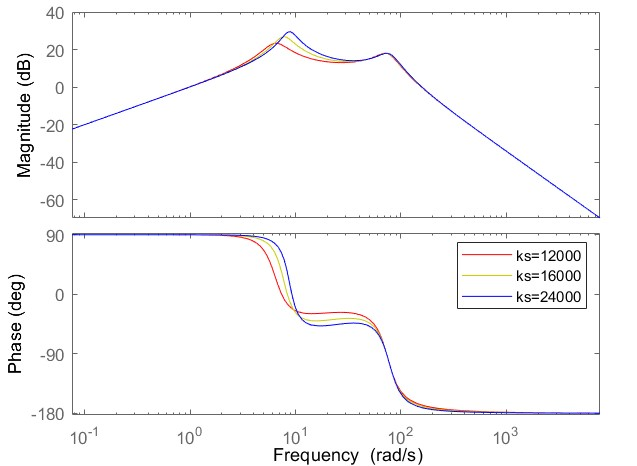
\includegraphics[width=.5\linewidth]{images/q2.2.3_a.jpg}}\hfill
        \subfloat[][Rattle Transfer Function Bode]{\label{fig:open_loop2_bode}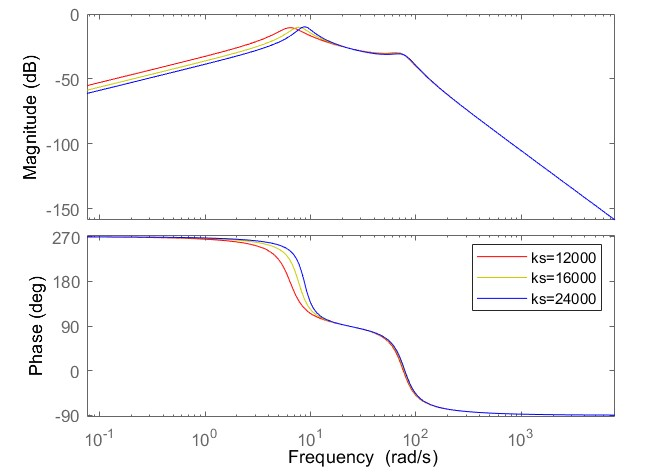
\includegraphics[width=.5\linewidth]{images/q2.2.3_b.jpg}}\hfill
        \subfloat[][Tyre Transfer Function]{\label{fig:open_loop3_bode}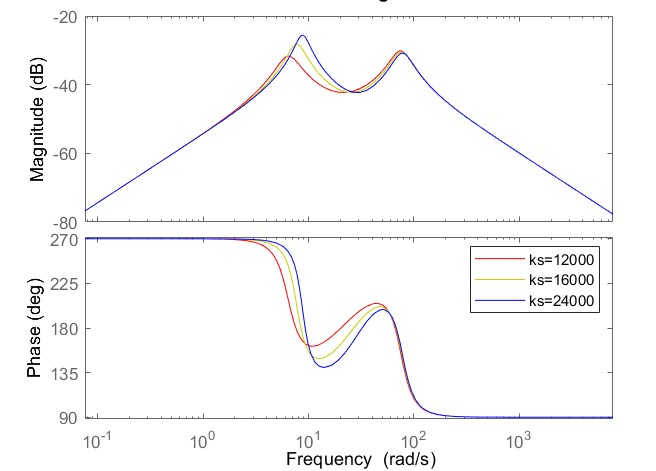
\includegraphics[width=.5\linewidth]{images/q2.2.3_c.jpg}}\par
        \caption{Bode plots of transfer functions for different suspension stiffness}
        \label{fig: open_loop_bode_ks}
    \end{figure}

    \textbf{Observations:}
    \begin{itemize}
        \item On observing the plots, the maxima of the plot occurs at higher frequencies as the
        suspension stiffness increases. So, natural frequencies increases with increase in suspension stiffness.
        \item As the stiffness increases, the ripples in the functions have steeper increase and decrease, indicating that the vehicle "jolts" more with increase in suspension stifiness.
        \item The decrease in relative stiffness between the suspension and the tyre as suspension
        stiffness increases, results ni an increased tyre deflection for higher values of suspension stiffness
    \end{itemize}

\subsection{Effect of Suspension Damping}


    For $b_s = 600 N/m$ 

    $A = \begin{bmatrix}
        0     & 1    & 0       & -1     \\
        -43.6 & -2.2 & 0       & 2.2    \\
        0     & 0    & 0       & 1      \\
        400   & 20.0 & -5333.3 & -20.0 
    \end{bmatrix}$\hfill \break

    For $b_s = 1000 N/m$ 

    $A = \begin{bmatrix}
        0     & 1    & 0       & -1      \\
        -43.6 & -3.6 & 0       & 3.6     \\
        0     & 0    & 0       & 1       \\
        400   & 23.33 & -5333.3 & -33.33 
    \end{bmatrix}$\hfill \break

    For $b_s = 1400 N/m$ 

    $A = \begin{bmatrix}
        0     & 1    & 0       & -1      \\
        -43.6 & -5.1 & 0       & 5.1     \\
        0     & 0    & 0       & 1       \\
        400   & 46.7 & -5333.3 & -46.7
    \end{bmatrix}$\hfill \break

    \textbf{Bode Plots:}
    \begin{figure}[H]
        \centering
        \subfloat[][Acceleration Transfer Function Bode]{\label{fig:open_loop1_bode}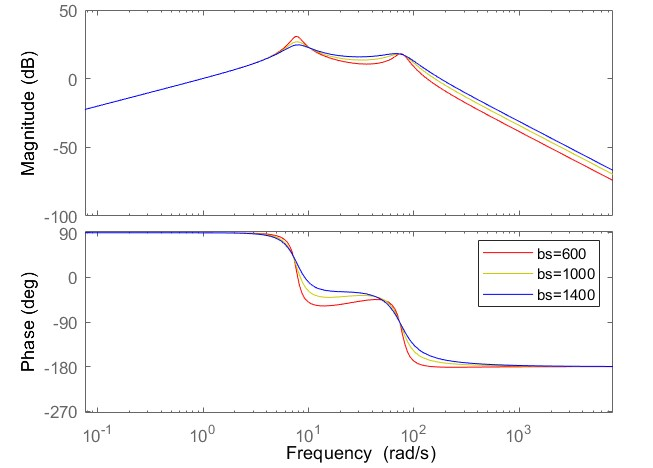
\includegraphics[width=.5\linewidth]{images/q2.2.4_a.jpg}}\hfill
        \subfloat[][Rattle Transfer Function Bode]{\label{fig:open_loop2_bode}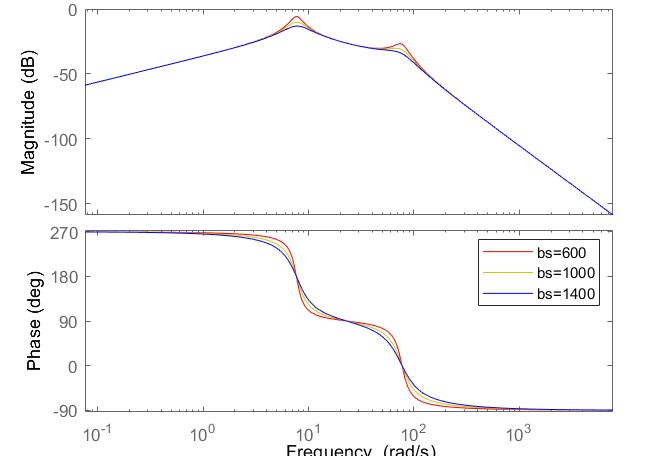
\includegraphics[width=.5\linewidth]{images/q2.2.4_b.jpg}}\hfill
        \subfloat[][Tyre Transfer Function]{\label{fig:open_loop3_bode}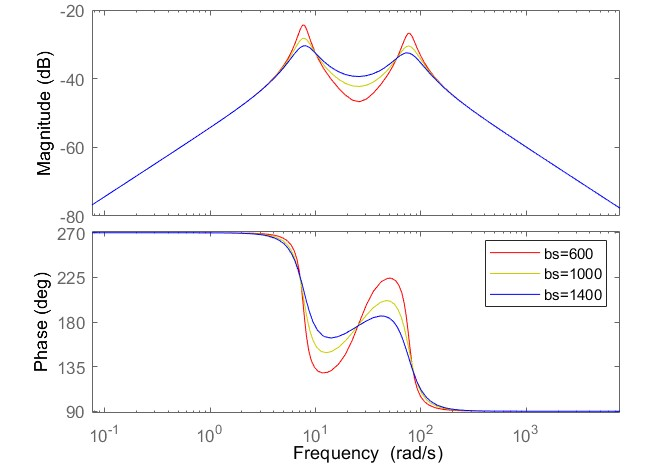
\includegraphics[width=.5\linewidth]{images/q2.2.4_c.jpg}}\par
        \caption{Bode plots of transfer functions for different suspension damping}
        \label{fig: open_loop_bode}
    \end{figure}

    \textbf{Observations:}
    \begin{itemize}
        \item As the peaks ofthe Bode plots occur at the same frequencies, the natural frequency of the system remains unaffected with the increase in damping values.
        \item The acceleration gains decrease as the damping increases, indicating the dampening out of irregularities. Also, the variations in the displacement functions are smoother with higher damping, meaning better smoothening of bumps.
        \item Higher suspension damping results in lesser variation in phase in case of the tyre deflection plot.
    \end{itemize}

\subsection{Effect of Tyre Stiffness}


    For $k_t = 100000 N/m$ 

    $A = \begin{bmatrix}
        0     & 1    & 0       & -1      \\
        -65.5 & -3.6 & 0       & 3.6     \\
        0     & 0    & 0       & 1       \\
        600   & 33.33 & -3333.3 & -33.33 
    \end{bmatrix}$\hfill \break

    For $k_t = 160000 N/m$ 

    $A = \begin{bmatrix}
        0     & 1    & 0       & -1      \\
        -65.5 & -3.6 & 0       & 3.6     \\
        0     & 0    & 0       & 1       \\
        600   & 33.33 & -5333.3 & -33.33 
    \end{bmatrix}$\hfill \break

    For $k_t = 200000 N/m$ 

    $A = \begin{bmatrix}
        0     & 1    & 0       & -1      \\
        -65.5 & -3.6 & 0       & 3.6     \\
        0     & 0    & 0       & 1       \\
        600   & 33.33 & -6666.7 & -33.33 
    \end{bmatrix}$\hfill \break

    \textbf{Bode Plots:}
    \begin{figure}[H]
        \centering
        \subfloat[][Acceleration Transfer Function Bode]{\label{fig:open_loop1_bode}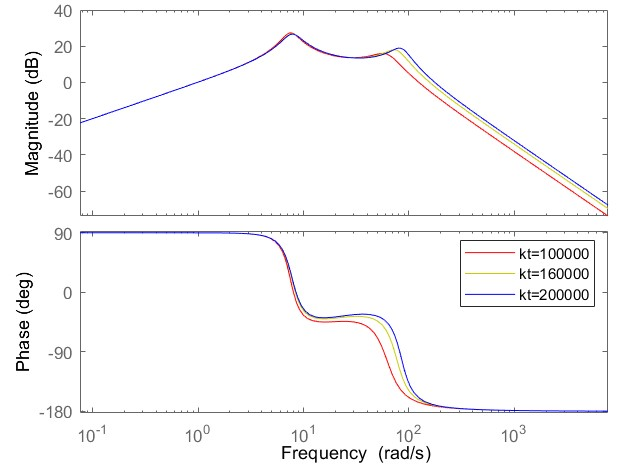
\includegraphics[width=.5\linewidth]{images/q2.2.5_a.jpg}}\hfill
        \subfloat[][Rattle Transfer Function Bode]{\label{fig:open_loop2_bode}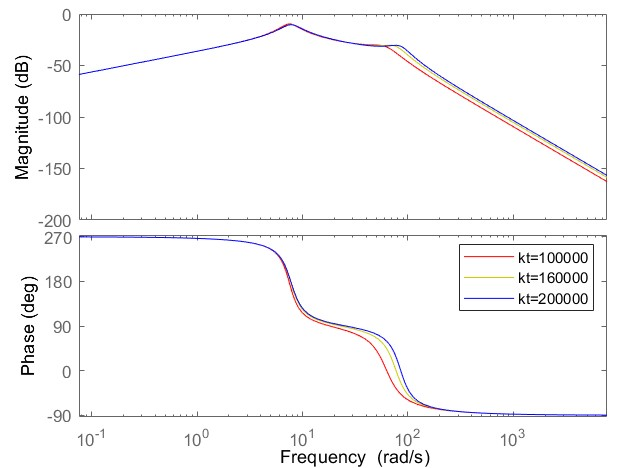
\includegraphics[width=.5\linewidth]{images/q2.2.5_b.jpg}}\hfill
    \end{figure}
    \begin{figure}[H]
        \centering
        \subfloat[][Tyre Transfer Function]{\label{fig:open_loop3_bode}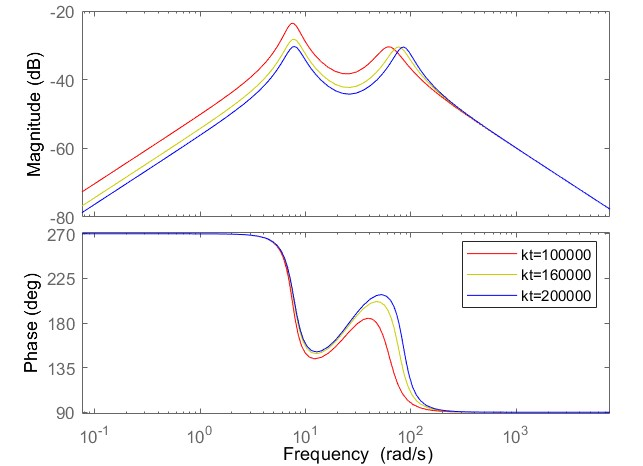
\includegraphics[width=.5\linewidth]{images/q2.2.5_c.jpg}}\par
        \caption{Bode plots of transfer functions for different suspension damping}
        \label{fig: open_loop_bode}
    \end{figure}

    \textbf{Observations:}
    \begin{itemize}
        \item The closed loop system reaches the steady state value much faster than that of open loop system.
        \item Also, for rectangular input in case of open loop system, the oscillation doesnot dies out, it keeps propagating as bundle of oscillations.
        \item The oscillations are decreased for the sprung mass case in closed loop system as compared to the open loop system and the ripples are smoothened as well to a larger extent
        \item The closed loop system is more stable.
    \end{itemize}

\chapter{Half Car Model}

\section{Governing Equations for Half Car Model}

\begin{figure}[h]
    \centering
    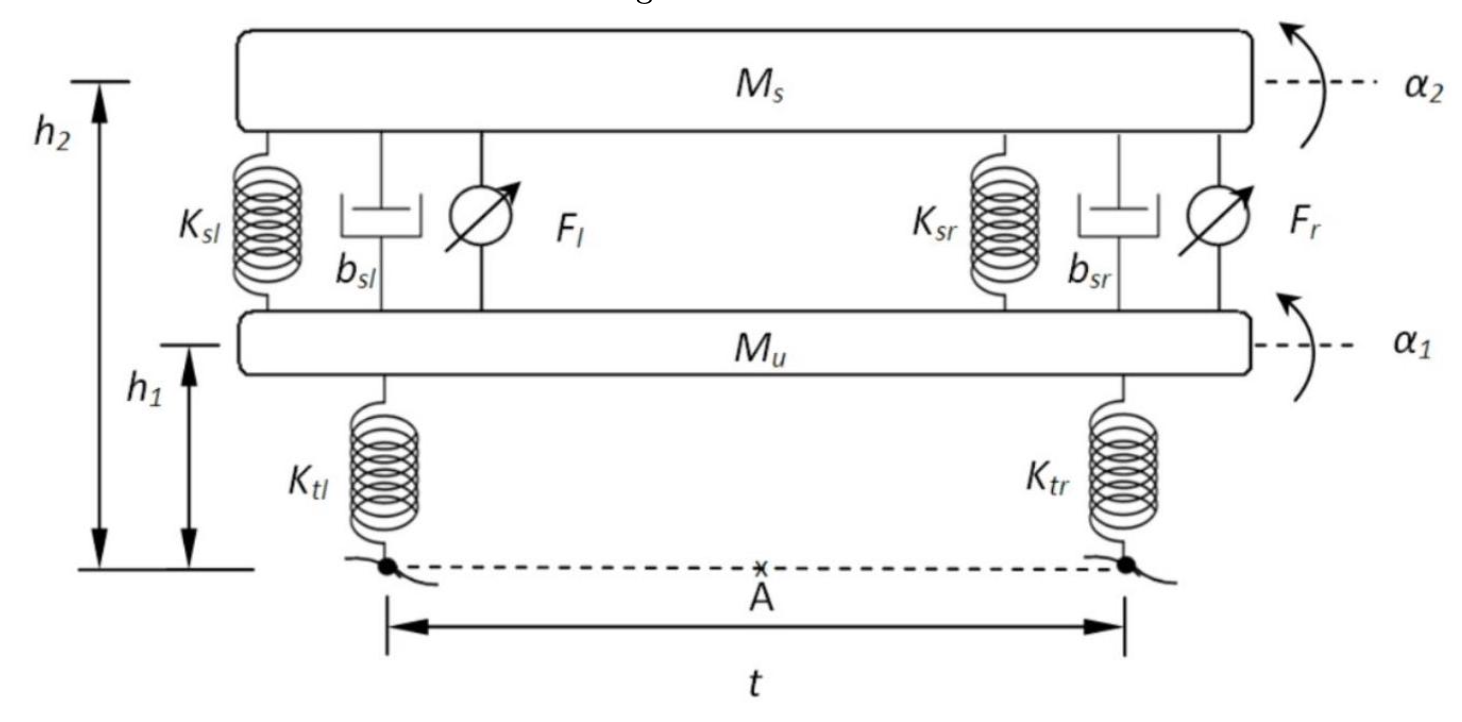
\includegraphics[width=0.5\textwidth]{images/Q4_halfcar_model.png}
    \caption{Half Car Model}
    \label{fig: half_car_model}
\end{figure}

\begin{itemize}
    \item  $M_s = \qty{1200}{kg}$: Sprung Mass
    \item $M_u = \qty{120}{ kg}$: Unsprung mass
    \item $k_{sl} = k_{sr} = \qty{50000}{N/m} $: Suspension stiffness
    \item $k_{tl} = k_{tr} = 350000 N/m$: Tyre stiffness
    \item $b_{sl} = b_{sr} = 3000 Ns/m$: Suspension damping 
    \item $t = 2.5m $: Track width
    \item $h_1 = 1 m $: Height of unsprung mass
    \item $h_2 = 2.2 m $: Height of sprung mass
    \item $I_s = 2000 kg (m)^2$: Sprung mass moment of inertia
    \item $I_u = 200 kg (m)^2$: Unsprung mass moment of inertia
\end{itemize}

\subsection{Equations of Motion}

\paragraph{Moment equation of unsprung mass about the roll point A},
\begin{multline}
        -k_{tr}\alpha_1 (t/2)^2 - k_{tl}\alpha_1 (t/2)^2 - F_{r} (t/2) + b_{sr}(\dot{\alpha_2} - \dot{\alpha_1}) (t/2)^2 \\ 
        + F_{l} (t/2) + k_{sl}(\alpha_2 - \alpha_1) (t/2)^2 + b_{sl}(\dot{\alpha_2} - \dot{\alpha_1})(t/2)^2 - m_u a_y h_1 = (I_u + m_u h_1^2) \ddot{\alpha_1}
\end{multline}

\paragraph{Moment equation of sprung mass about the roll point A},
\begin{multline}
    F_{r} (t/2) - b_{sr}(\dot{\alpha_2} - \dot{\alpha_1}) (t/2)^2  - k_{sr}(\alpha_2 - \alpha_1) (t/2)^2 - F_{l} (t/2) - k_{sl}(\alpha_2 - \alpha_1) (t/2)^2   \\ 
        - b_{sl}(\dot{\alpha_2} - \dot{\alpha_1})(t/2)^2 - m_s a_y h_2 = (I_s + m_s h_2^2) \ddot{\alpha_2}
\end{multline}

\section{State Space Model}

\begin{multline}
    \ddot{\alpha_1} = -\frac{(K_{sr} + k_{sl} + k_{tl} +k_{sl})}{I_u + m_u h_1^2} \alpha_1 + \frac{b_{sr}+b_{sl}}{I_u + m_u h_1^2} \dot{\alpha_1} + \frac{k_{sr} + k_{sl}}{I_u + m_u h_1^2}(t/2)^2 \alpha_2 + \frac{b_{sr}+b_{sl}}{I_u + m_u h_1^2}(t/2)^2 \dot{\alpha_1}\\
    + \frac{F_l}{I_u + m_u h_1^2}(t/2)- \frac{F_r}{I_u + m_u h_1^2}(t/2) - \frac{m_a a_y h_1}{I_u + m_u h_1^2}
\end{multline}

\begin{multline}
    \ddot{\alpha_2} = -\frac{(K_{sr} + k_{sl})}{I_s + m_s h_2^2} \alpha_1 + \frac{b_{sr}+b_{sl}}{I_s + m_s h_2^2} \dot{\alpha_1} + \frac{k_{sr} + k_{sl}}{I_s + m_s h_2^2}(t/2)^2 \alpha_2 + \frac{b_{sr}+b_{sl}}{I_s + m_s h_2^2}(t/2)^2 \dot{\alpha_2}\\
    + \frac{F_r}{I_s + m_s h_2^2}(t/2)- \frac{F_l}{I_s + m_s h_2^2}(t/2) - \frac{m_a a_y h_2}{I_s + m_s h_2^2}
\end{multline}

Considering the following as state variables,
\begin{equation}
    X = \begin{bmatrix}
        \alpha_1 \\
        \dot{\alpha_1} \\
        \alpha_2 \\
        \dot{\alpha_2}
    \end{bmatrix} ; 
    f(t) = \begin{bmatrix}
        F_l \\
        F_r
    \end{bmatrix}
\end{equation}
\begin{multline}
    \dot{X} = \begin{bmatrix}
        0 & 1 & 0 & 0 \\
        -\frac{(k_{sr} + k_{tr} + k_{tl} +k_{sl})}{I_u + m_u h_1^2}(t/2)^2 & -\frac{b_{sr}+b_{sl}}{I_u + m_u h_1^2}(t/2)^2 & \frac{k_{sr} + k_{sl}}{I_u + m_u h_1^2}(t/2)^2 & \frac{b_{sr}+b_{sl}}{I_u + m_u h_1^2}(t/2)^2 \\
        0 & 0 & 0 & 1 \\
        \frac{(k_{sr} + k_{sl})}{I_s + m_s h_2^2}(t/2)^2 & \frac{b_{sr}+b_{sl}}{I_s + m_s h_2^2}(t/2)^2 & -\frac{k_{sr} + k_{sl}}{I_s + m_s h_2^2} & -\frac{b_{sr}+b_{sl}}{I_s + m_s h_2^2}(t/2)^2
    \end{bmatrix} X \\
    + \begin{bmatrix}
        0 & 0 \\
        -\frac{t/2}{I_u + m_u h_1^2} & \frac{t/2}{I_u + m_u h_1^2} \\
        0 & 0 \\
        \frac{t/2}{I_s + m_s h_2^2} & -\frac{t/2}{I_s + m_s h_2^2}
    \end{bmatrix} f(t) 
    + \begin{bmatrix}
        0 \\
        -\frac{m_u h_1}{I_u + m_u h_1^2} \\
        0 \\
        \frac{m_s h_2}{I_s + m_s h_2^2}
    \end{bmatrix} a_y
    \label{eq:state_space_model_halfcar}
\end{multline}

Comparing the the above equation \ref{eq:state_space_model_halfcar}, we have

\begin{align*}
    A & = \begin{bmatrix}
        0 & 1 & 0 & 0 \\
        -\frac{(k_{sr} + k_{tr} + k_{tl} +k_{sl})}{I_u + m_u h_1^2}(t/2)^2 & -\frac{b_{sr}+b_{sl}}{I_u + m_u h_1^2}(t/2)^2 & \frac{k_{sr} + k_{sl}}{I_u + m_u h_1^2}(t/2)^2 & \frac{b_{sr}+b_{sl}}{I_u + m_u h_1^2}(t/2)^2 \\
        0 & 0 & 0 & 1 \\
        \frac{(k_{sr} + k_{sl})}{I_s + m_s h_2^2}(t/2)^2 & \frac{b_{sr}+b_{sl}}{I_s + m_s h_2^2}(t/2)^2 & -\frac{k_{sr} + k_{sl}}{I_s + m_s h_2^2} & -\frac{b_{sr}+b_{sl}}{I_s + m_s h_2^2}(t/2)^2
    \end{bmatrix} \\
    & = \begin{bmatrix}
        0 & 1 & 0 & 0 \\
        -3906.2 & -29.3 & 488.3 & 29.3 \\
        0 & 0 & 0 & 1 \\
        20 & 1.2 & -12.8 & -1.2
    \end{bmatrix}
\end{align*}
\begin{equation*}
    B = \begin{bmatrix}
        0 & 0 \\
        -\frac{t/2}{I_u + m_u h_1^2} & \frac{t/2}{I_u + m_u h_1^2} \\
        0 & 0 \\
        \frac{t/2}{I_s + m_s h_2^2} & -\frac{t/2}{I_s + m_s h_2^2}
    \end{bmatrix} 
    = \begin{bmatrix}
        0 & 0 \\
        -0.0039 & 0.0039 \\
        0 & 0 \\
        0.0002 & -0.0002
    \end{bmatrix}
\end{equation*}
\begin{equation*}
    d = \begin{bmatrix}
        0 \\
        -\frac{m_u h_1}{I_u + m_u h_1^2} \\
        0 \\
        \frac{m_s h_2}{I_s + m_s h_2^2}
    \end{bmatrix}
    = \begin{bmatrix}
        0 \\
        0.0038 \\
        0 \\
        2.0613
    \end{bmatrix} \times 10^{7}
\end{equation*}

\section{Performance Index}

We define the performance index as the following:
\begin{equation}
    J = \int_{0}^{t_f} \left( \rho_1 \alpha_1^2 + \rho_2 \dot{\alpha_1}^2 + \rho_3 \alpha_2^2 + \rho_4 \dot{\alpha_2}^2 + \rho_4 F_r^2 + \rho_4 F_l^2  \right) dt
\end{equation}
This can be written as:
\begin{equation}
    J = \int_{0}^{\infty} \left( x^T Q x + 2 x^T n f + f^T R f \right) dt
\end{equation}

where $Q$ is the state cost matrix, $R$ is the input cost matrix, $n$ is the input cost vector, and $x$ is the state vector.

Given weights $\begin{bmatrix}
    \rho_1 & \rho_2 & \rho_3 & \rho_4 & \rho_5 & \rho_6
\end{bmatrix} = \begin{bmatrix}
    16 & 16 & 40000 & 16 & 10^{-9} & 10^{-9}
\end{bmatrix}$
\begin{equation*}
    Q = \begin{bmatrix}
        \rho_1 & 0 & 0 & 0 \\
        0 & \rho_2 & 0 & 0 \\
        0 & 0 & \rho_3 & 0 \\
        0 & 0 & 0 & \rho_4
    \end{bmatrix} ;
    R = \begin{bmatrix}
        \rho_5 & 0 \\
        0 & \rho_6
    \end{bmatrix} ;
    n = \begin{bmatrix}
        0 & 0 \\
        0 & 0 \\
        0 & 0 \\
        0 & 0
    \end{bmatrix}
\end{equation*}

Calculating using MATLAB, we get

\begin{figure}[h]
    \centering
    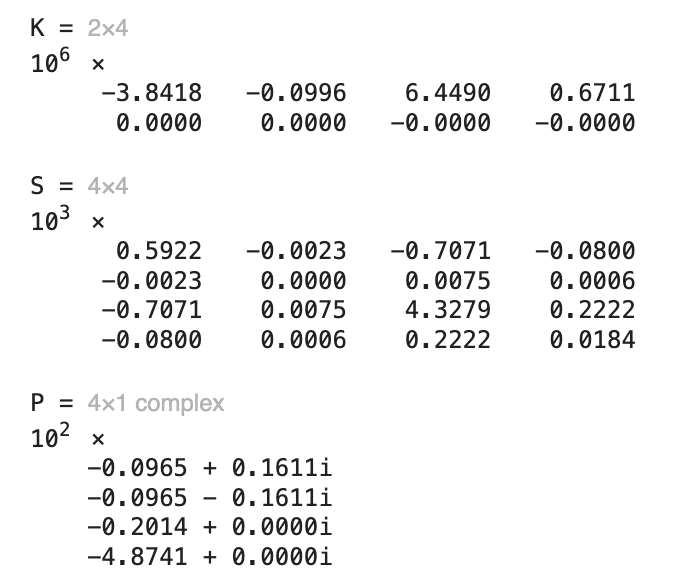
\includegraphics[width=0.5\linewidth]{images/Q4_LQR.png}
    \caption{LQR Parameters}
    \label{fig:Q4_LQR}
\end{figure}

\section{Active and Passive Suspension Comparison}

\subsection{Passive Suspension}

For passive suspension, $ \dot X = A X + d a_y $

\begin{equation}
    \alpha_1 (s) = \frac{38400 s^2 + 6.039e08 s + 1.007e10}{38400 s^2 + 6.039e08 s + 1.007e10}
    \label{eq:Q4_passive_alpha1}
\end{equation}

\begin{equation}
    \alpha_2 (s) = \frac{2.061e07 s^2 + 6.039e08 s + 8.052e10}{2.061e07 s^2 + 6.039e08 s + 8.052e10}
\end{equation}

\begin{figure}[h]
    \centering
    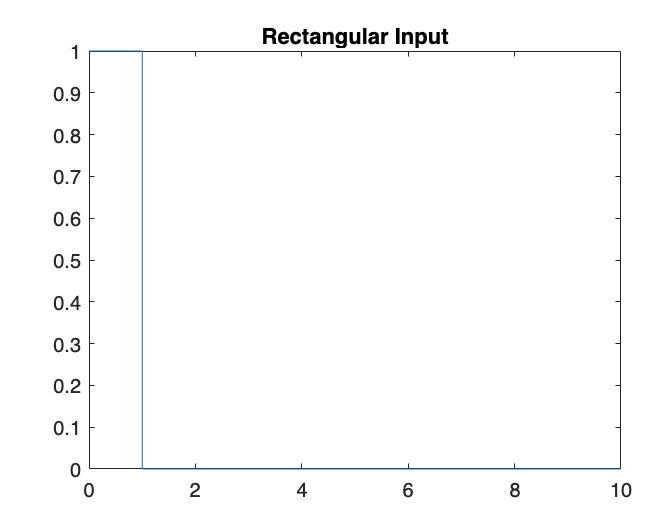
\includegraphics[width=0.5\linewidth]{images/Q4_step_input.png}
    \caption{Step Input}
    \label{fig:Q4_step_input}
\end{figure}

\begin{figure}[h]
    \subfloat[Passive Suspension Impulse Response]{\label{fig:Q4_passive_impulse}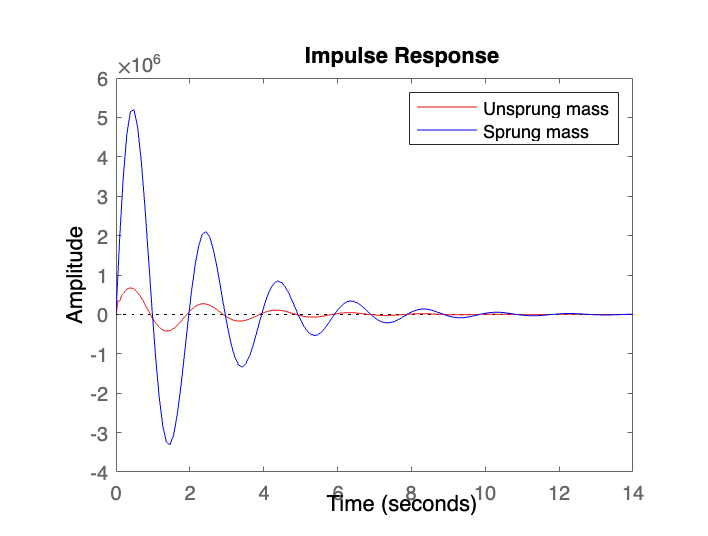
\includegraphics[width=.5\linewidth]{images/Q4_passive_impulse.png}}\hfill
    \subfloat[Passive Suspension Step Response]{\label{fig:Q4_passive_step}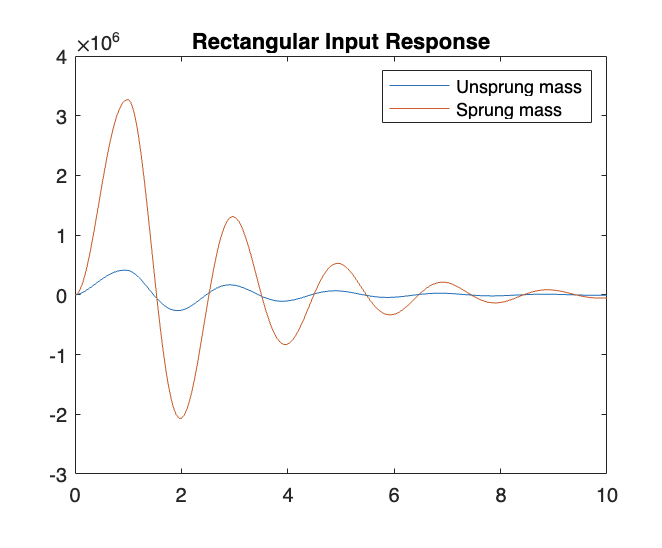
\includegraphics[width=.5\linewidth]{images/Q4_passive_step.png}}\par 
    \caption{Passive Suspension Responses}
    \label{fig:Q4_passive_responses}
\end{figure}

\section{Active Suspension}

For active suspension, $ \dot X = A X + B f(t) + d a_y $

From LQR Control, we obtain $K$. Hence, $f = -K X$.
Therefore, $ \dot X = A X + B (-K X) + d a_y $ = $ (A - B K) X + d a_y $

Hence, $ A_{cl} = A - B K = \begin{bmatrix}
    0 & 1 & 0 & 0 \\
    -1891.3 & -41.8 & 2568 & 265.1 \\
    0 & 0 & 0 & 1 \\
    63.5 & 1.7 & -104.5 & -10.9
\end{bmatrix}$

The new transfer function will be,
\begin{equation}
    \alpha_1 (s) = \frac{3.84e04 s^2 + 5.464e10 s + 5.294e11}{ s^4 + 526.8 s^3 + 1.996e04 s^2 + 3.683e05 s + 3.461e06}
    \label{eq:Q4_active_alpha1}
\end{equation}

\begin{equation}
    \alpha_2 (s) = \frac{2.061e07 s^2 + 8.621e09 s + 3.899e11}{2.061e07 s^2 + 8.621e09 s + 3.899e11}
    \label{eq:Q4_active_alpha2}
\end{equation}

\begin{figure}[h]
    \centering
    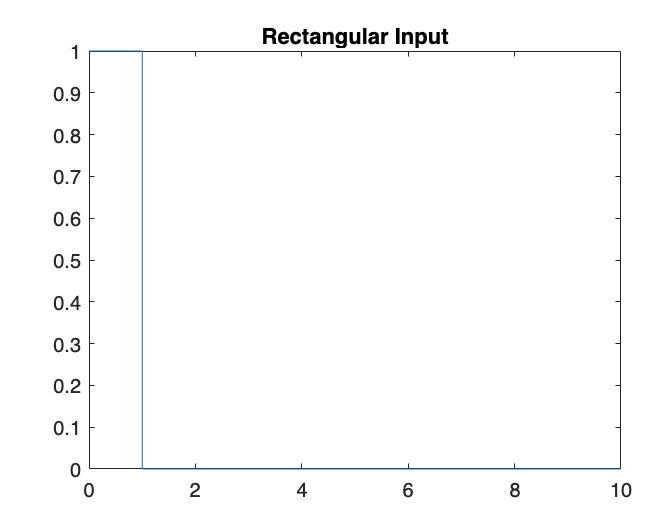
\includegraphics[width=0.5\linewidth]{images/Q4_step_input.png}
    \caption{Step Input}
    \label{fig:Q4_step_input}
\end{figure}

\begin{figure}[h]
    \subfloat[Active Suspension Impulse Response]{\label{fig:Q4_active_impulse}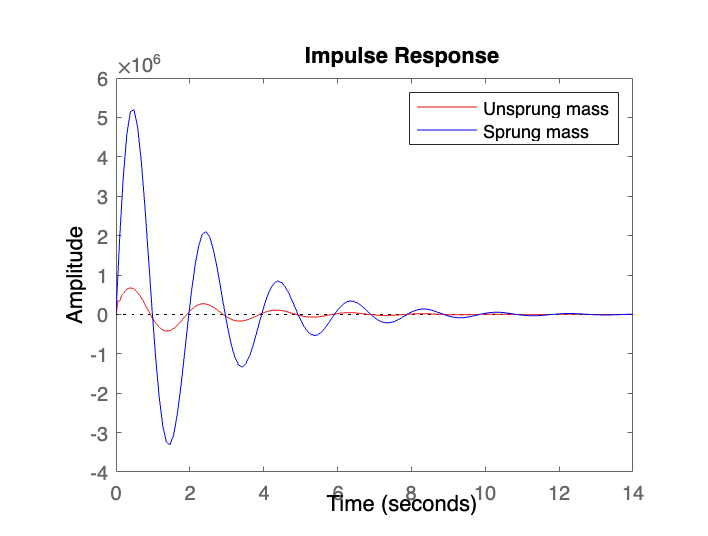
\includegraphics[width=.5\linewidth]{images/Q4_passive_impulse.png}}\hfill
    \subfloat[Active Suspension Step Response]{\label{fig:Q4_active_step}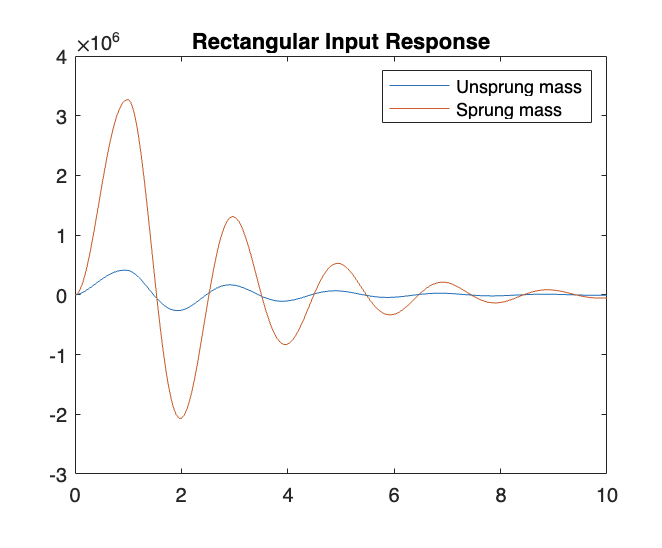
\includegraphics[width=.5\linewidth]{images/Q4_passive_step.png}}\par 
    \caption{Active Suspension Responses}
    \label{fig:Q4_active_responses}
\end{figure}



\chapter{Conclusion}

We have successfully derived the dynamic bicycle model using state space representation and converted it into transfer function. We have also designed a controller for the system using root locus method. We have also seen the effect of longitudinal speed on the system.

\end{document}


